
\section{QoI Model}
\label{sec:qoi_model}

The utility of data that is extracted from a sensor or military tactical network is often highly dependent on the context of the data with respect to aspects like the network's goals and the other data being collected from the network.  While this effect is often very qualitative by nature, we introduce metrics here that provide real examples of how QoI can be measured quantitatively.  These measures are based on the similarity or dissimilarity between images and will be used as examples in the QoI-aware network scalability in Section \ref{sec:qoi_scalability}.  

\subsection{Image Similarity}

First, we must establish a practical method of measuring the similarity of two images.  To do so, we can use qualities inherent to a photograph like lightness, contrast, and color.  Many techniques have been studied to compare photographs with these qualities.  We choose to use one such technique called Color and Edge Directivity Descriptor (CEDD) \cite{2008cedd}.  With CEDD, each image is described by a vector of 144 different features describing color and spatial color distribution.  

Using this CEDD feature vector of each image, we can compare any two images.  To achieve a scalar representation of similarity, from comparing two vectors, we use \emph{Tanimoto similarity}, which is commonly considered in the image processing community \cite{tanimoto}, $T_s$. The Taminoto similarity metric is defined as follows. Given two images with feature vectors $\mathbf{a}$ and $\mathbf{b}$,
  \begin{equation}
  T_s(\mathbf{a,b})=\frac{\mathbf{a.b}}{\mathbf{a.a+b.b-a.b}},
  \end{equation}
where $\mathbf{a.b}$ is the inner product of two vectors. Proper normalization keeps this metric in the $[0,1]$ range. Naturally, to describe the dissimilarity, or distance, of two photographs, then, we simply use $T_d = 1 - T_s$.

\subsection{Image Selection Algorithms}

As a motivating example, we choose a mobile network in which nodes generate photographs that are to exchanged or collected at one or more data sinks.  This example covers surveillance missions of military tactical networks or civilian/social scenarios, one example of which could be smartphone users contributing to an image-sharing application.  We will provide two example scenarios of using content-based image selection that will motivate the algorithms used and results generated in this work.

The first application occurs when a user would like to find more images that are similar to one already obtained.  For example, if a user observes a picture of an unknown suspicious person entering a building, but the person is not identifiable from that image, it would be useful to collect more images that are similar to that one with the possibility that another picture of the building from another user may have a better view of the person in question that can be used for identification or more context.  In a social situation, a user may want more views of a particular event of interest like a parade or a concert.  Called \emph{Top-K}, the algorithm used for this application will choose the $k$ images with the smallest distance from the given image. 

The second application we introduce is called a \emph{spanner}, and it is based on an opposing scenario.  Instead of  choosing matching images, the goal of a spanner is to select the $k$ images that exhibit the most joint dissimilarity.  This algorithm would be useful in a surveillance mission or other setting in which a user would like to get a snapshot of all areas of which photographs were taken that is as complete as possible.  

\subsection{Measuring QoI}

As already discussed, \emph{Quality of Information} is a very contextual term, so defining metrics to provide objective measurements of it is a challenge within itself.  Here, we provide two different methods of calculating scores for completeness or diversity being achieved.  

With both the Top-K and Spanner algorithms, initial choices exhibit higher degrees of similarity and dissimilarity, respectively, that naturally decrease.  Therefore, if we establish a measure of overall QoI being obtained as $k$ is increased, we witness an effect of diminishing returns.  For the Top-K algorithm, we define \emph{Sum Similarity}, which is the cumulative sum of the similarity score of each image being selected.  

For the spanner algorithm, we employ a greedy algorithm similar to that in \cite{mediascope} to simplify implementation and to define a \emph{Sum Dissimilarity} metric.  Here, the algorithm first chooses the two images with the greatest distance between them from all available images.  Then, each successive image is chosen to be the one with the greatest minimum distance between it and all images already chosen, until $k$ images are selected.  This minimum distance between the image being selected and the images in the collected set is the value added to the running QoI metric of \emph{Sum Dissimilarity}.

Figures \ref{fig:topkSumSim} and \ref{fig:spanSumDissim} shows the diminishing returns of using similarity and dissimilarity metrics.  This effect is important also because it visually shows how Quality of Information differs from throughput.  As these graphs clearly show, transmission of successive images is not linear in terms of gained completeness.  Inversely, this relationship shows that obtaining a certain value of QoI or completeness may require a different number of images depending on the set available and their similarities.  Specifically, we can denote the number of images required to achieve a level of completeness, $S$, as $N(S)$.  This relationship will be useful later in determining feasible scalability.

%Top-k Sum Similarity
\begin{figure} 
\begin{centering}
    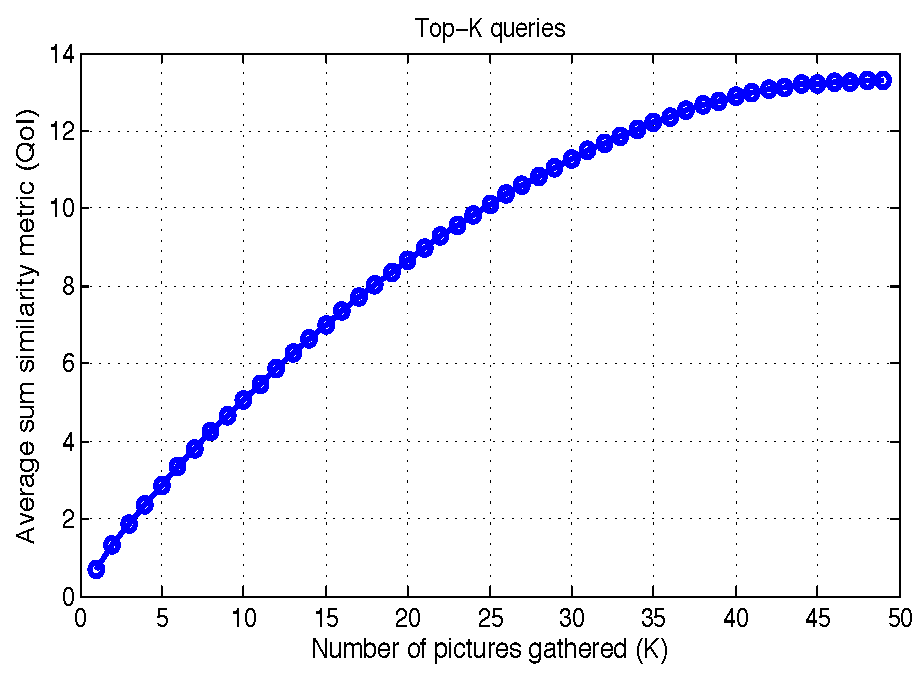
\includegraphics[scale=0.45]{figures/topkSumSimilarity.pdf}
    \caption{Sum Similartiy for Top-K Results of Varying $k$}
    \label{fig:topkSumSim}
\end{centering}
\end{figure}

%Spanner Cumulative Distance
\begin{figure} 
\begin{centering}
    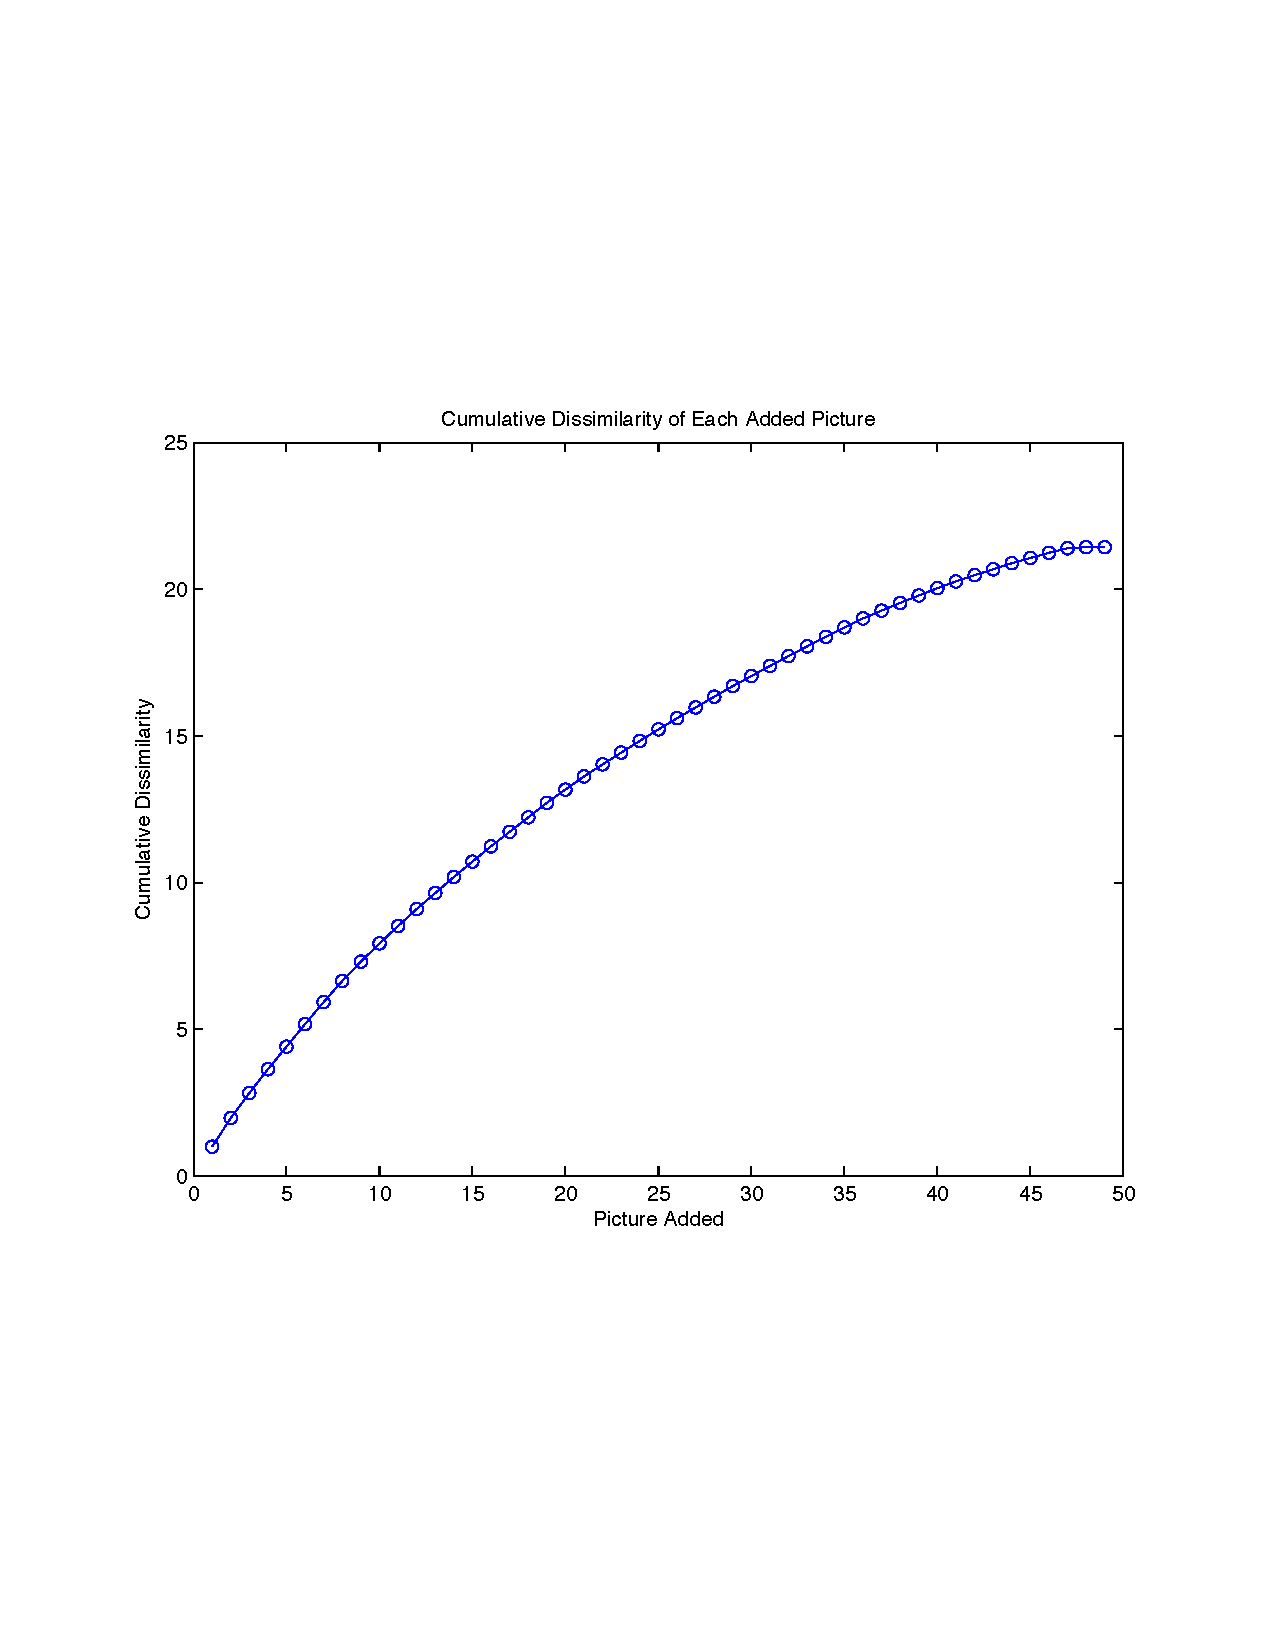
\includegraphics[scale=0.35]{figures/spannerCumulativeDist.pdf}
    \caption{Sum Dissimilarity for Spanners of Varying $k$}
    \label{fig:spanSumDissim}
\end{centering}
\end{figure}

To provide a second approach to measuring QoI, we can use a model in which each image belongs to one of $n$ sets, $Q_n$, which can each represent a particular setting of interest.  Naturally, then, when executing a Top-K query, the goal is for the algorithm to return images from the same set as the target image.  In the case of a spanner query, the goal is to return images from different sets.  

Using these two naturally-occuring goals, we can measure the effectiveness of the algorithms, providing QoI values.  For Top-K, the QoI value is the number of photographs returned that are in the same set as the target image.  For the spanner algorithm, the QoI value can either be the number of sets covered by at least one of the returned images, or it can be the likelihood that all $n$ sets will be covered by the returned images, as long as $k \geq n$.

To provide example values of these QoI metrics, experiments were run on photographs taken at $5$ different settings around the Penn State campus.  Each of the settings is of a pictorially different setting, e.g. a particular building, a downtown street, or a lawn setting, and over $20$ images of each was taken.  Then, for individual trials, sets of $Q_n$ with $10$ images in each set were randomly selected from this group of photographs and the Top-K and spanner algorithms were run over these $50$ images with the target image being randomly selected in the case of Top-K.

Figures \ref{fig:topkAvgNumSameSet}-\ref{fig:spannerAvgNumSetsCov} show the average results of 1000 trials.  In Figure \ref{fig:topkAvgNumSameSet}, it is evident that a value of only $k \approx 10$ is needed to collect $5$ images matching the target content, while collecting an additional $2$ from the same usually requires collecting over twice the number of pictures.  

This diminishing return is also evident in the spanner algorithm results.  Figure \ref{fig:spannerAvgNumSetsCov} shows the number of sets represented by the algorithm output for increasing $k$.  Here, if the goal is to achieve at least one image from each of the different settings as might be in a surveillance application, the spanner achieves it on average at $k \approx 17$.  The same trend is evident in Figure \ref{fig:spannerAvgPercAllSetsCov} where the probability of covering all sets is plotted against $k$.  Using this metric, the application can use the probability of achieving full coverage as the QoI metric.  From this example application, if collecting at least one image from each set with $90\%$ probability of success is acceptable, then only $k=13$ images are necessary.

% Top-K Average Number from Same Set Returned
\begin{figure} 
\begin{centering}
    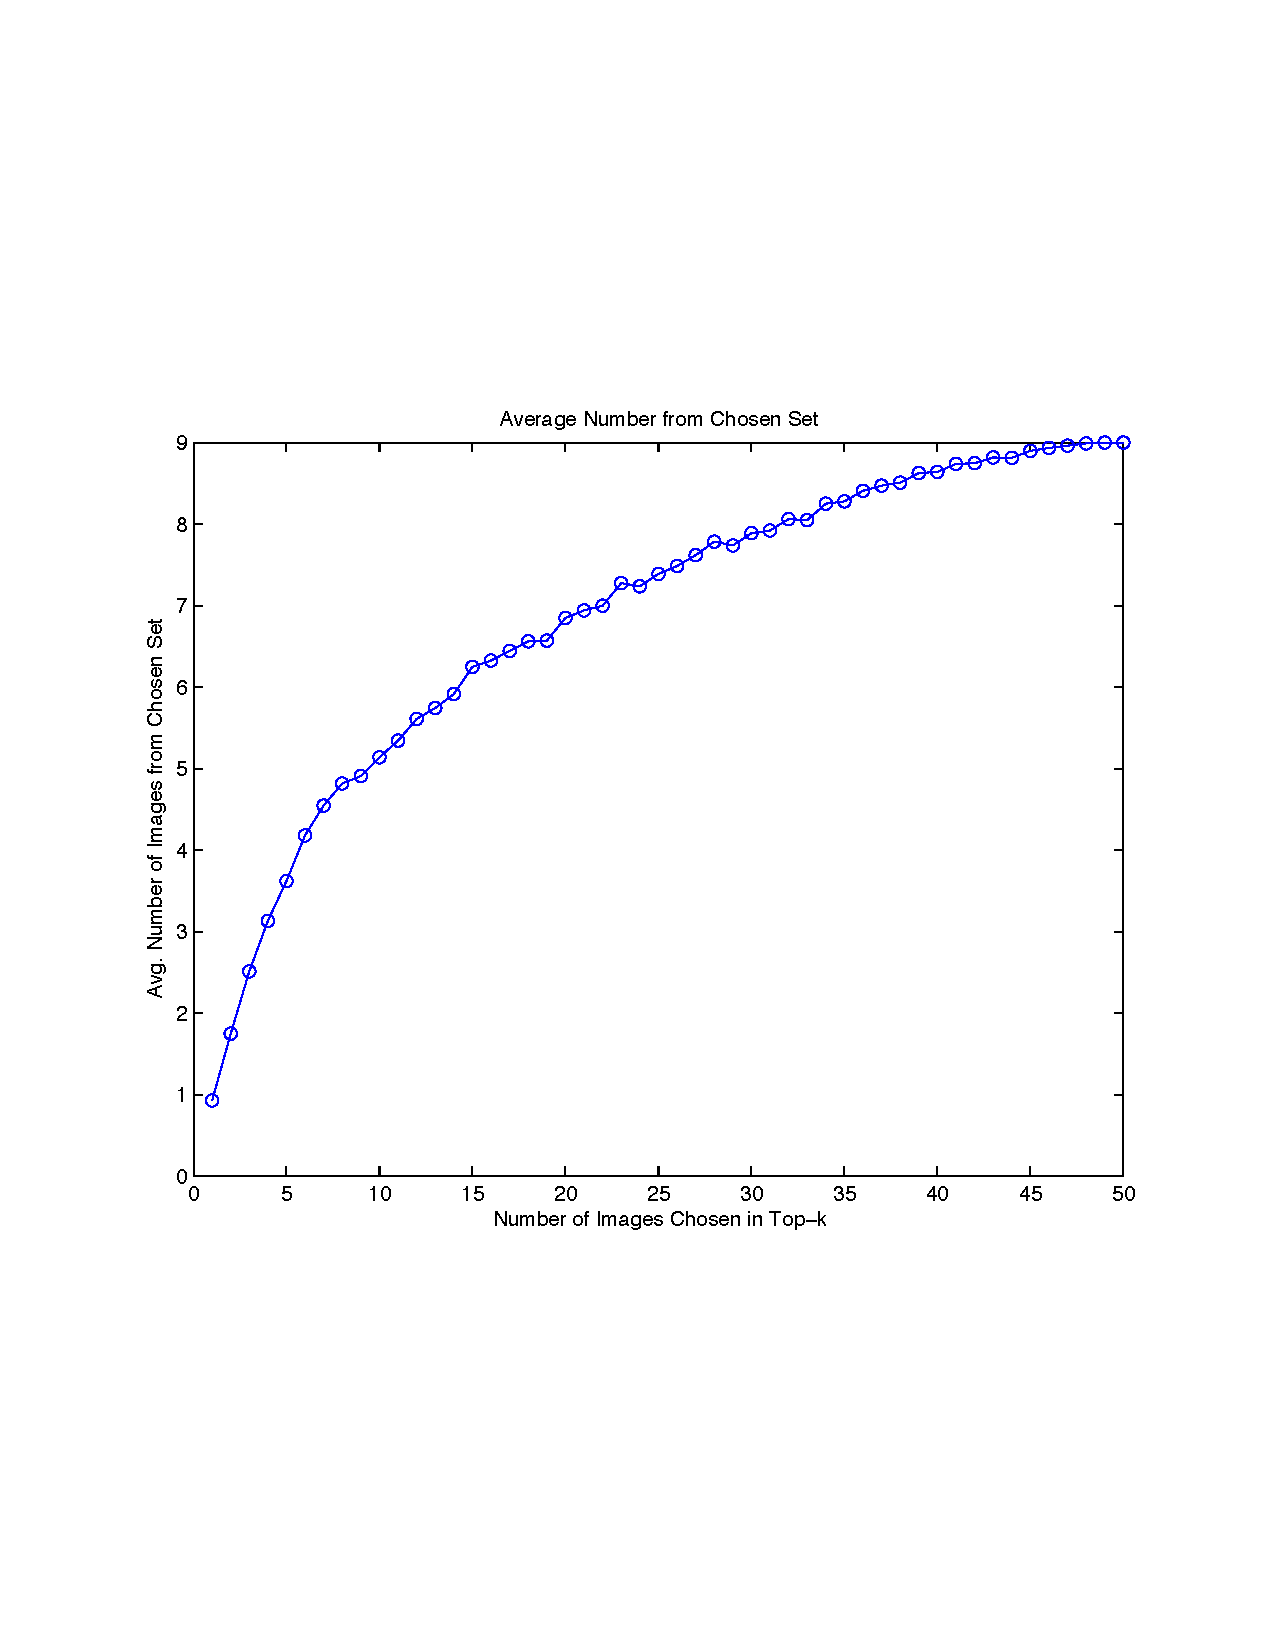
\includegraphics[scale=0.35]{figures/50_image_sets/avgNumMatching_50_images.pdf}
    \caption{Average Number of Images Selected from Same Set as Target Image}
    \label{fig:topkAvgNumSameSet}
\end{centering}
\end{figure}

% Spanner Average Number Sets Covered
\begin{figure} 
\begin{centering}
    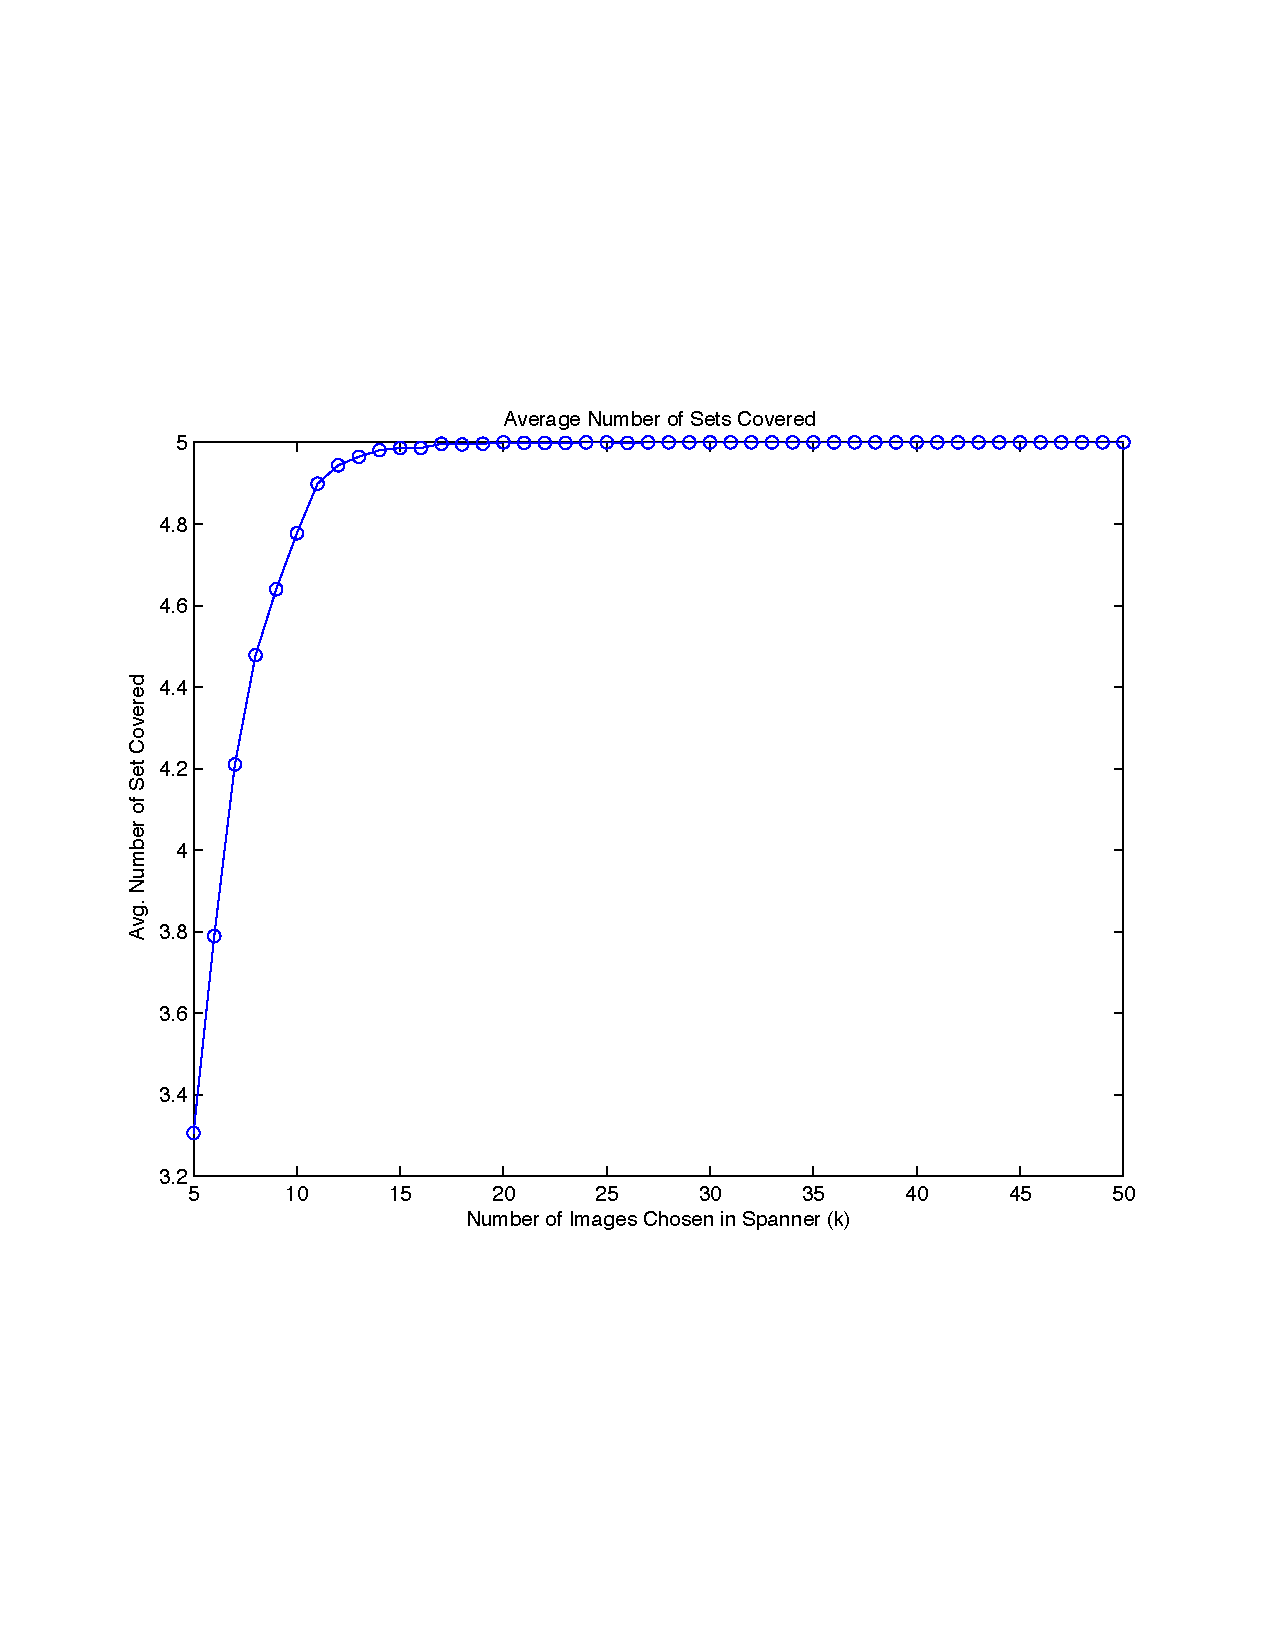
\includegraphics[scale=0.35]{figures/50_image_sets/percCoverage_50_images.pdf}
    \caption{Average Number of Sets Covered by Returned Images}
    \label{fig:spannerAvgNumSetsCov}
\end{centering}
\end{figure}

% Top-K Average Number from Same Set Returned
\begin{figure} 
\begin{centering}
    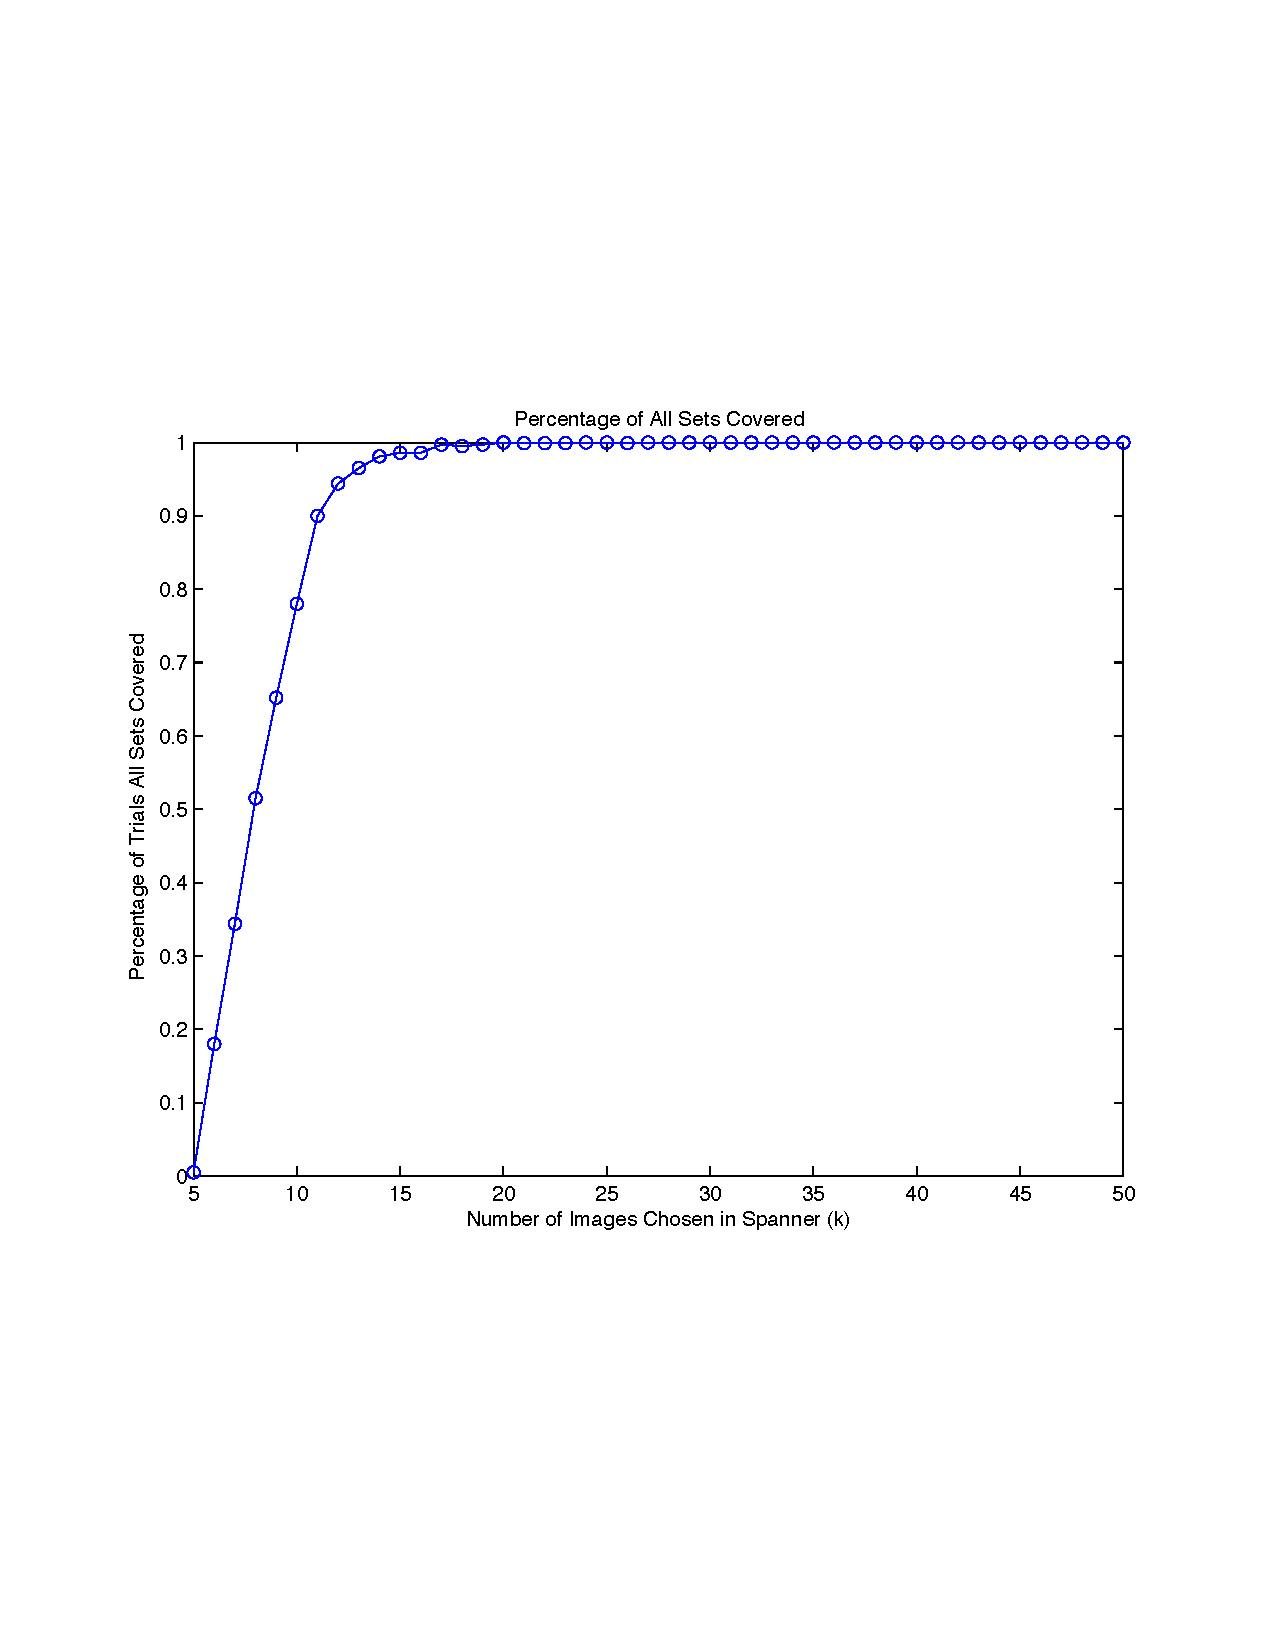
\includegraphics[scale=0.35]{figures/50_image_sets/percAllSetsCovered_50_images.pdf}
    \caption{Average Percentage All Sets Covered by Returned Images}
    \label{fig:spannerAvgPercAllSetsCov}
\end{centering}
\end{figure}



%As for how we were planning to relate a notion of QoI which is increasing with more images;
%The Top_K query seems readily expandable for different K-you give a target image and as you collect more images you add more "similarity metrics"(which reduces with distances), but the spanner had some issues:
%If normalized among all distances, the average distance among elements reduces with more elements.
%On the other hand, if we simply add pairwise distances, it overcounts too many combinations (n choose 2)
%So, the latest possibility I had in mind was to consider an additive metric such that each introduced picture brings increases the metric proportion to either the avg distance to existing elements, or minimum/maximum of all distances to the existing elements. 
%Given the definition of "spanner", which is "Spanner maximizes the minimum dissimilarity between all pairs", what  I had in mind was perhaps to consider an additive metric such that each introduced picture increases the metric proportion to the minimum of all distances to the existing elements. Or, since the whole set of selected pictures might change with different 
%K, probably the best metric is:
%
%For a spanner of K pictures: Total "quality/diversity metric" = \sum_{i=1 to K} min_{j in K-i} (distance_i, j)
%
%that is, we run the spanner, find K pictures. For each picture we have a minimum dissimilartity/distance to rest of the pictures. Than, we add these minimum dissimilarities over all pictures. 
%I think the case where the extra metric added is in proportion to the average distances should decrease for each new added picture, so we should have a increasing concave type function.

%the graph is generated as follows: 
%given a timeliness T and dissimilarity(D)/similarity(S) requirement, we find how many nodes the network can scale up to, say N, by the scalability analysis formulas.
%Then we look at how many images are required for attaining D/S, say K(this comes from the CEDD based MATLAB analysis). With the assumption that each node has one image, this essentially implies a lower bound on the required network size in terms of number of nodes to attain D/S.
%If N<K, the network cant actually scale large enough to provide the similarity/dissimilarity, so it is not "scalably feasible".
%so this graph is obtained as follows; for each T, identify the largest D/S such that N>=K still holds.
